%!TEX root = ../thesis.tex
\chapter{Quad-tree mesh in 2D analysis}
\label{qdt_sec:main}
\section{Introduction}
\paragraph{}
The main objective of this chapter is to introduce a way that can utilize the engineering design available in the AutoCAD or other popular commercial softwares for 2D cases.
The data format that used in almost all engineering design softwares that can represent the geometry exactly is IGES file.
It will be used as a bridge between design and numerical analysis.
%
\paragraph{}
After the NURBS information representing the exact geometry has been extracted from the IGES file, the quad-tree mesh generation algorithm described in \ref{qt_sc:quadtree} will be adopted to generate a high quality mesh.
Either the NURBS basis functions or the traditional shape functions can be used as the shape function of the SBFEM solver.
% We further extend the method to problems with singularities within the framework of linear elastic fracture mechanics.
The proposed method enhances the conventional SBFEM and the salient features of the method are:
    \begin{itemize}
        \item No human effort involvement in mesh generation
        \item Retained exact geometry
        \item High quality mesh generated from the quad-tree algorithm
    \end{itemize}
\paragraph{}
This chapter is organized as follows.
The CAD output (iges files) will be introduced first.
After that, an overview of the algorithm that can generate quadtree mesh will be provided.
Furthermore, a point projection which project intersection point back to the NURBS surface is presented.
The accuracy and the convergence properties of the proposed techniques are demonstrated with benchmark problems in the context of linear elasticity, followed by concluding remarks in the last section.
\pagebreak

\section{CAD output in 2D}
\label{qt_sc:iges}
\paragraph{}
The IGES\cite{IGES1983} files introduced in Sec.~\ref{lr_sec:IGES} are used as the bridge between the engineering design and the numerical analysis in the proposed method.
As a standard file format in engineering design industry, it is supported by almost all design softwares all over the world.
Consequently, it offers a possibility to minimize the human effort spent on mesh generation.

\subsection{Parse geometry in IGES file}
\paragraph{}
The IGES file provides all information that describe the geometric input.
Abstract structure of the IGES file that describe the 2D geometry can be regarded as a simple curve-surface structure.
In other words, it defines the geometric input as certain number of surfaces with their boundaries in different colors, which represent different materials in engineering practice.
Each surface contains a list of curve indices which are corresponding to the curve information described in IGES file.

\paragraph{}
When the IGES file is feed into the programme, each line in the directory entry will be parsed entity by entity.
Parameter in directory entry describe the type and reference to other useful values for the entity.
An entity may refer to one or many entities in directory entry.
Detail of the specification of each entity is explained in \cite{Nasr2007} in detail.

%=====================================================================================================================%
\subsection{Output to mesh generator}
\label{qdt_section:iges_output}
\paragraph{}
The output file that the mesh generator read in will be a shorter summary of the geometric input.
Boundary representation will be kept as the data structure to describe the geometric input.
However, some fields apart from the curves or the surfaces will be added.
In the output file, the geometry will be organized in key points, polylines and surfaces.
The key points define the coordinates of all points and polylines are used to represent all curves including NURBS curves for simplification.
NURBS curves introduced in in \ref{lr_sec:NURBS} can be used directly by the mesh generator as well but it is found that the computational cost in the calculation of the distance between points to NURBS curves surpasses the merits of using it directly.
The exact geometry can be retained by projecting the nodes on the boundary back to the origin NURBS curves at the end of the algorithm.

\paragraph{}
Representing a straight line with polyline can be natural, first and the last points will be enough to achieve an exact representation.
However, that is not the case for curves whose curvature is not always zero.
Although adding more key points can increase the quality of polyline representation, computational cost in calculating the distance increases at the same time.
Yet, having only few key points may result in a bad polyline representation which leads to a poor mesh quality.
Elements may be twisted after the nodes on the boundary are projected to the origin curves.
As a consequence, a quantified indicator that is able to control the number and the position of the vertices on the polyline can be necessary.

%=====================================================================================================================%
\subsection{Discretization of the circular arc}
\paragraph{}
The chord ratio can be a good indicator for circular arc.
The arc length to chord length ratio $\frac{a}{L}$ illustrated in Fig.~\ref{qt_fig:iges_chord_ratio} can be expressed in angle $\alpha$ as:
    \begin{equation}
        \frac{a}{L} = \frac{
            \sqrt{2-2\cos\alpha}
        }{\alpha}
        = \frac{
            2\sin\frac{\alpha}{2}
        }{\alpha}
    \end{equation}
%
The maximum angle $\alpha$ satisfy arc length to chord length ratio $\frac{a}{L} > 1-\epsilon$ with $
    \sin\frac{\alpha}{2} = 1 - \frac{x^3}{6} + O(x^7)
$ can be derived as:
    \begin{equation}
        \alpha < \sqrt{24 \epsilon}
    \end{equation}

    \begin{figure}[h!]
        \centering
        \scalebox{1}{
            \includegraphics{quadtree/images/iges_chord_ratio.eps}
        }
        \caption{Chord length for circular arc}
        \label{qt_fig:iges_chord_ratio}
    \end{figure}
%
%=====================================================================================================================%
\subsection{Discretization of the NURBS curve}
\paragraph{}
For NURBS curves who have no closed form chord ratio, similar idea can be applied numerically.
The NURBS curve is first divided into serval smaller ones based on the knot vector as described in Sec.~\ref{lr_sec:nurbs_knot_ins}.  % may be explained in detail
Since the order of each subdivided NURBS curve used in engineering softwares are predominantly lower or equal to three, the sub-curves then can be divided into two classes, convex curves or concave curves with an inflection point as shown in Fig.~\ref{qt_fig:iges_chord_ratio_nurbs}.
    \begin{figure}
        \begin{subfigure}[b]{0.5\linewidth}
            \centering
            \scalebox{0.5}{
                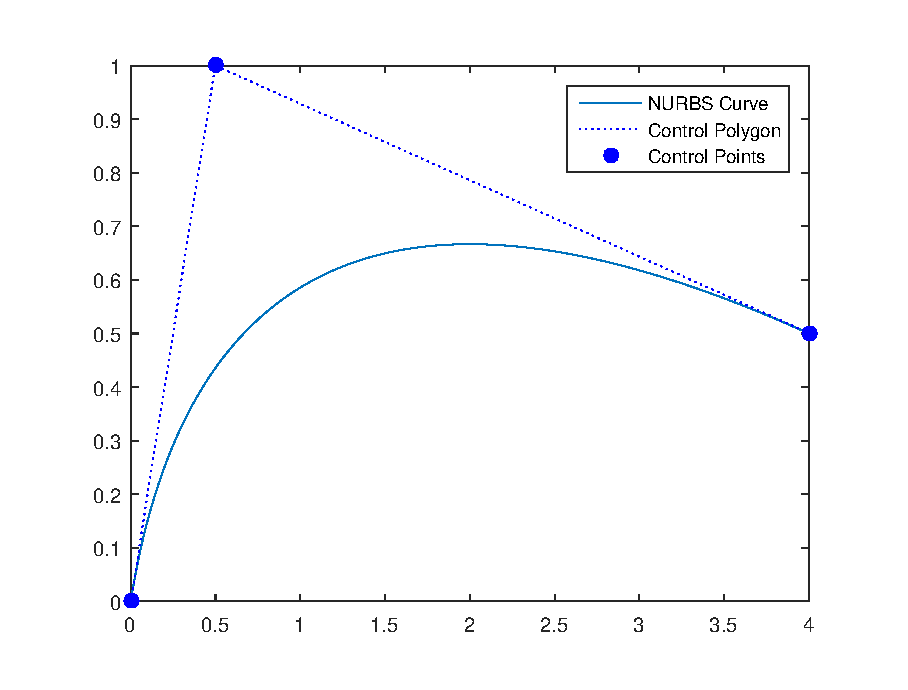
\includegraphics{quadtree/images/iges_chord_ratio_nurbs_convex.eps}
            }
            \caption{Convex}
        \end{subfigure}
        \begin{subfigure}[b]{0.5\linewidth}
            \centering
            \scalebox{0.5}{
                \includegraphics{quadtree/images/iges_chord_ratio_nurbs_concave.eps}
            }
            \caption{Concave with an inflection point}
        \end{subfigure}
    \caption{Type of sub-devided NURBS curves: convex and concave with an inflection point}
    \label{qt_fig:iges_chord_ratio_nurbs}
    \end{figure}
%
In order to determine the target NURBS curve is convex one or concave one, a cross product will be conducted.
by assuming the subdivided NURBS curve is cubic, there will be four control points $P_1,P_2,P_3$ and $P_4$.
If the signs of $cross(\overrightarrow{P_1P_2},\overrightarrow{P_2P_3})$ and $cross(\overrightarrow{P_1P_2},\overrightarrow{P_2P_3})$ are the same, then the curve is convex.
Otherwise it will be concave.

%=====================================================================================================================%
\subsubsection{Convex curves}
\label{qt_ssc:convex_curves}
\paragraph{}
Start with the simple case, in the situation illustrated in Fig.~\ref{qt_fig:iges_chord_split_convex_sum} where line $C(u_0)C(u_n)$ and the NURBS curve form a convex set, we are looking for a point $C(u_m)$ on the curve so that $C'(u_m)$ is parallel to $\overrightarrow{C(u_0)C(u_n)}$
    \begin{figure}[h!]
        \centering
        \scalebox{0.6}{
            \includegraphics{quadtree/images/iges_chord_split_convex_sum.eps}
        }
        \caption{Discretization for convex NURBS curve}
        \label{qt_fig:iges_chord_split_convex_sum}
    \end{figure}
%
The target is to split one NURBS curve segment into two.
The splitting will be processed until the arc length to chord length ratio of any splitted curves are smaller than the tolerance.
Based on the property of the convex set, there can be one and only one parameter $u_m$ that satisfies the condition.
As a consequence, numerical methods such as Newton's method can be adopted to determine it.
For a given $u_m$, the next iteration will be:
    \begin{equation}
        u_{m_{new}} =  u_n - \frac{f(u_m)}{f'(u_m)}
    \end{equation}
%
where 
    \begin{equation}
        f(u) = C'(u) \begin{bmatrix}
            - C_y(u_n) + C_y(u_0) \\
            C_x(u_n) - C_x(u_0)
        \end{bmatrix}
    \end{equation}
%
The procedure to find $u_m$ can be concluded in Algorithm.~\ref{qdt_alg:split_convex_nurbs} and Algorithm.~\ref{qdt_alg:discrete_convex_nurbs} describes the procedure to find all knots corresponding to the vertexes of the polylines recursively.
\begin{algorithm}
    function splitConvexCurve(curve,u\_0, u\_n) \\
    \Input{
        curve, the input NURBS curve \\
        u\_0,u\_n, two end knots of the NURBS curve
    }
    \Output{
        u\_m, in Fig.~\ref{qt_fig:iges_chord_split_convex_sum}
    }
    u\_m = (u\_n + u\_0) * 0.5 \\
    pt\_0, pt\_n = getCurvePts(u\_0, u\_n) \\
    vector\_0n = Vector(pt\_0,pt\_n) \\
    angle = vector\_0n.atan2() \\
    deri1\_m = getCurveDeri(u\_m,1) \\
    angle\_m = deri1\_m.atan2() \\
    \While{abs(angle\_m-anlge)$<10^{-4}$}
      {
        deri1\_m, deri2\_m = getCurveDeri(u\_m,2) \\
        angle\_m = atan2(deri1\_m.y, deri1\_m.x)  \\
        fu = deri1\_m * vector\_0n.normalVector() \\
        fu\_deri = deri2\_m * vector\_0n.normalVector() \\
        u\_m = u\_m - fu / fu\_deri \\
        deri1\_m = getCurveDeri(u\_m,1) \\
        angle\_m = deri1\_m.atan2()
      }
    \caption{Split a convex NURBS curve into two}
    \label{qdt_alg:split_convex_nurbs}
\end{algorithm}
%
%
\begin{algorithm}
    function discreteConvexCurve(curve,eps,u\_0,u\_n,u)
    \Input{
        curve, the input NURBS curve \\
        eps, the tolerance of the chord to arc-length ratio \\
        u\_0,u\_n, two end knots of the NURBS curve
    }
    \Output{
        u, the vector of the knot corresponding to vertexes of the polylines
    }
    arcLength = curve.arcLength(u\_0,u\_n) \\
    chordLength = curve.getPt(u\_0).distanceTo(curve.getPt(u\_n)) \\
    \eIf{1-chordLength/arcLength $<$ eps}{
        return
    }{
        u\_m = (splitConvexCurve(curve,u\_0,u\_n))
        u.add(u\_m)
        discreteConvexCurve(curve,eps,u\_0,u\_m)
        discreteConvexCurve(curve,eps,u\_m,u\_n)
        return
    }    
\caption{Discrete a convex NURBS curve recursively}
\label{qdt_alg:discrete_convex_nurbs}
\end{algorithm}
%=====================================================================================================================%
\subsubsection{Concave curves}
\paragraph{}
As can be seen in Fig.~\ref{qt_fig:iges_chord_ratio_nurbs}, the extracted cubic NURBS curve will have no more than one inflection point.
The reason for that is because the target function is cubic and hence its second derivative will be in first order.
Consequently, numerical methods such as Newton's method can be used to find this unique point.
After that, the curve can be divided into two convex ones and the algorithms introduced in \ref{qt_ssc:convex_curves} can be used separately.
The Newton's iteration can be written as
    \begin{equation}
        u_{n_{new}} = u_n - \frac{f(u_n)}{f'(u_n)}
    \end{equation}

where
    \begin{equation}
        f(u) = C''(u)
    \end{equation}
%
%=====================================================================================================================%
\subsubsection{Calculation of the arc length}
\paragraph{}
The arc length of the NURBS curve defined on $u \in [u_0, u_n]$ can be expressed as
    \begin{equation}
        L = \int_{u_0} ^{u_n} \sqrt{C_x^2(u) + C_y^2(u)} du
    \end{equation}
%
The integration can be solved by the help of the numerical integration quadrature described in \ref{iso_section:numerical_integration} as:
    \begin{equation}
        L = \sum_{i=0}^n a_i \sqrt{C_x^2(u_i) + C_y^2(u_i)}
    \end{equation}


\section{Quad-tree structure}
\label{qt_sc:quadtree}
\paragraph{}
After the geometry information is exported from the IGES file, it can be feed into the quad-tree algorithm to generate mesh of the problem domain.
As an algorithm based on computational geometry, it require great amount of numerical operation and hence the result may be sensitive to the tolerance.
An absolute tolerance may not be able to handle problem with very large or small geometric size.
As a consequence, the first step is to normalize the geometry into a uniform space ($10\times10$ is used in this chapter).

\subsection{Background mesh}
\paragraph{}
Background mesh, like its name, describe a mesh in the background. %fig
Its density is decided by the geometry.
This section will introduce the procedure to generate the background mesh.
\paragraph{}
First of all, we start with one square which is the root of the tree.
The size of it will be slightly larger than the normalized input geometry and it is selected as $16 \times 16$ in this chapter.
After that, the root square will be divided into millions (defined by resolution, defined as $2^{res} \times 2^{res}$) smaller ones like pixel in the image.
Then, $2^{s_{max}} \times 2^{s_{max}}$ pixels will be group into the first layer of the tree, or initial background mesh.
It is used to control the maximum allowable mesh size globally or separately for different material regions.
There are two ways to decided whether each individual square need to be refined or not, seed points method and curve size field and both of them will be used depends on the requirement of the controlling over the mesh.

\paragraph{}


\subsection{Hardpoint treatment}

\subsection{Bucket sort algorithm}

\subsection{Cutting with boundary}

\subsection{Color the region}


\section{Points projection}
\label{qt_sc:projection}
\subsection{Projection algorithm}
\paragraph{}
Point projection algorithm is to find the nearest point in parameter $(u)$ on the NURBS curve of the test point.
In the proposed method, all points on the NURBS curve is generated based on the approximated polylines and hence are not exactly on the boundaries.
Although there exists a closed form solution for point projection, it require the order of the NURBS curve must be less than $4$ \citep{Pie1997}.
As a consequence, a projection algorithm \citep{MA200379} using Newton-Raphson method is introduced to tackle this problem.

\paragraph{}
For a given point $P=(x,y)$, its projection on the curve $C(u$ so that the distance $|P-C(u)|$ is minimum is targeted.
However, in the proposed method, the existence of the large number of the possible curves increase the computational cost significantly.
The projection point for the test point $P$ need to be determined for every existing curves and the one with the smallest minimum distance will be selected.
One possible improvement could be limit the possible curves to only a few by utilizing the fact that the NURBS curves has been divided into multiple sub-curves without interior knot by knot insertion introduced in Sec.~\ref{lr_sec:nurbs_knot_ins}
Another property that can be utilized is that most of the test point $P$ is expected to be extremely close to its projection on the curve $C(u)$.

\paragraph{}
As a consequence, the strong convex hull property can be adopted to limit the number of possible curves to less than $2$.
The building of the convex hull is explained in detail in Sec.~\ref{qdt_sc:convex_hull}.
The signed distance of the test point to all curves' convex hull is calculated and only the curves with negative signed distance which indicate that the point is in the convex hull will be selected as candidates.
If no negative distance is detected, a few number (taken as $3$ in the proposed method) of curves with minimum signed distance will be selected.

\paragraph{}
In order to find the projection of the test point $P$ on the curve $C$, target function $f$ can be expressed as
\begin{equation}
    f(u) = \mathbf{C}^\prime (u) \cdot (\mathbf{C}(u) - \mathbf{P})
\end{equation}
%
When $f(u)$ gives $0$, the point either located on the curve or the distance $|\mathbf{C}(u) - \mathbf{P}|$ is minimal.
and two scalars $f$ and $g$ are defined as
%
The iteration can be concluded as
\begin{equation}
    u_{i+1} = u_i -
    \frac{ f(u_i) }{ f^\prime(u_i) }
\label{qdt_eq:projection_iteration}
\end{equation}
After one iteration is finished, the following criteria are checked in sequence.
\paragraph{1}
Is the point coincide with $C(u_i)$
\begin{equation*}
    |\mathbf{C} (u_i) - \mathbf{P}| \leq \epsilon_1
\end{equation*}
%
where $\epsilon_1$ stands for the tolerance for distance in Euclidean space.
\paragraph{2}
Is the cosine zero
\begin{equation*}
    \frac{
        |\mathbf{C}^\prime (u) \cdot (\mathbf{C}(u) - \mathbf{P})|
    }{
        |\mathbf{C}^\prime (u)|
        |\mathbf{C}(u) - \mathbf{P}|
    } \leq \epsilon_2
\end{equation*}
%
where $\epsilon_2$ stands for the tolerance for cosine.
If either of these conditions are met, the iteration is terminated.
Otherwise Eq.~\ref{qdt_eq:projection_iteration} is performed to find the parameter $u_{i+1}$ for next iteration.
\paragraph{3}
Make sure $u$ and $v$ are within there domains
\begin{equation*}
    u_{i+1} \in [a,b]
\end{equation*}
%
where $a$ and $b$ are the lower and upper bounds for the knot vector of curve $C$.
If the curve is open
\begin{equation}
    \left\{
        \begin{array}{rl}
            u_{i+1} = a & u_{i+1} < a \\
            u_{i+1} = b & u_{i+1} > b
        \end{array}
    \right.
\end{equation}
%
If the curve is closed
\begin{equation}
    \left\{
        \begin{array}{rl}
            u_{i+1} = b - ( a - u_{i+1} ) & u_{i+1} < a \\
            u_{i+1} = a + ( u_{i+1} - b ) & u_{i+1} > b
        \end{array}
    \right.
\end{equation}
%
\paragraph{4}
The difference between the new parameter $u_{i+1}$ and the old one $u_i$ is insignificant
\begin{equation*}
    |
        (u_{i+1} - u_i)\mathbf{C}^\prime(u_i)
    |
    \leq \epsilon_1
\end{equation*}
The iteration will be terminated if this condition is meet.



\subsection{Convex hull in 2D}
\label{qdt_sc:convex_hull}
\paragraph{}
The convex hull property of the NURBS curve indicates that all points on the curve must be contained within the convex hull constructed by its control points \citep{SELIMOVIC2009772}
There are great number of algorithm that can be used including gift wrapping \citep{Cormen:2009:IAT:1614191}, graham scan \citep{ANDERSON197853}, quick hull \citep{Barber:1996:QAC:235815.235821}, Chan's algorithm \citep{Chan1996} and so on \citep{doi:10.1137/0215021, ANDREW1979216}.
The quick hull is adopted in the proposed as it provides a computationally efficient and stable algorithm.
The algorithm utilize the idea of `` divide and conquer'' to build the convex hull with an expected time complexity of $O(nlog(n))$ and  $O(n^2)$ for the worst case.
Generally speaking, it works as expected in most of the situation except for the case of high symmetry or most of the points located at the circumference of a circle.
The algorithm can be implemented with following steps:
\begin{enumerate}
    \item Find the most left and right points (points with minimal and maximum $x$) since they are proved to be part of the convex hull.
    \item Connect these two points and use the line to separate other points into two group.
    \item Find the point with maximum distance to the line in step 2 in any group.
    \item Construct a triangle with two points in step 2 and the point in step 3.
    \item Eliminate all points contained by these two subsets in step 4.
    \item Repeat the previous three steps and the distance calculated in step 2 is determined as the point to the triangle instead of the line in step 1.
    \item Terminate the iteration when no points are left
\end{enumerate}


\section{Numerical Examples}
\subsection{Cantilever beam}
\paragraph{}
A two-dimensional cantilever beam subjected to a parabolic shear load at the free end is examined as shown in Fig.~\ref{qdt_fig:ex_cantilever_beam_geo_bc}.
    \begin{figure}[h!]
    \centering
        \scalebox{0.6}{\includegraphics{isogeometric_sbfem/images/cantilever_beam_geo_bc.eps}}
        \caption{ Cantilever beam: Geometry and boundary conditions.}
        \label{qdt_fig:ex_cantilever_beam_geo_bc}
    \end{figure}
%
The geometry is: length $L=8m$, height $D=4m$.
The material properties are: Young’s modulus $E$ = $3 \times 10^7 N/m^2$ , Poisson’s ratio $ \nu =0.25$.
The parabolic shear force is $P = 250 N$.
The exact solutions for the displacements are given by \citep{Aug2008} as Eq.~\ref{iso_eq:cantilever_beam_displacement_solution}.
where $I=D^3/12$ is the moment of inertia, $\mean{E}=E$, $\mean{\nu}=\nu$ and $\mean{E}=E/(1-\nu^2)$, $\mean{\nu}=nu/(1-nu)$ for plane stress and plane strain condition respectively.
The stress $\sigma$ can be expressed as \citep{Aug2008} as Eq.~\ref{iso_eq:cantilever_beam_stress_solution}.
The strain energy can be derived from Eq.~\ref{iso_eq:cantilever_beam_stress_solution} and Eq.~\ref{iso_eq:cantilever_beam_displacement_solution} as Eq.~\ref{iso_eq:cantilever_beam_energy_solution}.

\paragraph{}
In this example, rigid body motion is constrained by fixing 3 DOF on the left edge of the beam.
$u_x=0$ for points at $(0,-D/2)$ and $(0,D/2)$ and $u_y =0$ for point at $(0,0)$.
Stress from analytical solution in Eq.~\ref{iso_eq:cantilever_beam_stress_solution} are applied on the boundaries.

\paragraph{}
Due to the fact that the geometry of the cantilever beam can be described by four points and four straight lines, drawing in AutoCAD may not be necessary.
As a result, the input geometry is defined manually.
Generated background mesh, coloring and the final result with $res=32$, $s_{max}=16$ and $s_{min}=1$ are shown in Fig.~\ref{qdt_fig:ex_cantilever_beam_background_mesh}, Fig.~\ref{qdt_fig:ex_cantilever_beam_mesh_coloring} and Fig.~\ref{qdt_fig:ex_cantilever_beam_mesh_final}.

    \begin{figure}
        \centering
        \scalebox{0.4}{
            \includegraphics{quadtree/ex_images/cantilever_background_mesh.eps}
        }
        \caption[Background mesh of cantilever beam]{Background mesh of cantilever beam : Bold lines represents the input geometry}
        \label{qdt_fig:ex_cantilever_beam_background_mesh}
    \end{figure}

    \begin{figure}
        \centering
        \scalebox{0.4}{
            \includegraphics{quadtree/ex_images/cantilever_coloring.eps}
        }
        \caption[Mesh coloring of cantilever beam]{Mesh coloring of cantilever beam : Grey area represents the cantilever beam}
        \label{qdt_fig:ex_cantilever_beam_mesh_coloring}
    \end{figure}

    \begin{figure}
        \centering
        \scalebox{0.3}{
            \includegraphics{quadtree/ex_images/cantilever_final_mesh.eps}
        }
        \caption[Final mesh of cantilever beam]{Final mesh of cantilever beam}
        \label{qdt_fig:ex_cantilever_beam_mesh_final}
    \end{figure}
% DOF err
% 146 - 0.019587 (32,16)
% 178 - 0.0082845 (32,2)
% 438 - 0.0027044 (64,2)
% 1658- 0.00066929 (128,2)
Mesh with different parameters are plotted in Fig.~\ref{qdt_fig:ex_cantilever_mesh_all} and the convergence study is plotted in Fig.~\ref{qdt_fig:ex_cantilever_mesh_conv}

    \begin{figure}[h!]
        \begin{subfigure}[b]{1\linewidth}
            \centering
            \scalebox{0.4}{
                \includegraphics{quadtree/ex_images/qdt_cantilever_mesh_178.eps}
            }
            \caption{Mesh with $res=32$, $s_{max}=2$, 178 DOFs}
        \end{subfigure}
        \\
        \begin{subfigure}[b]{1\linewidth}
            \centering
            \scalebox{0.4}{
                \includegraphics{quadtree/ex_images/qdt_cantilever_mesh_438.eps}
            }
            \caption{Mesh with $res=64$, $s_{max}=2$, 438 DOFs}
        \end{subfigure}
        \\
        \begin{subfigure}[b]{1\linewidth}
            \centering
            \scalebox{0.4}{
                \includegraphics{quadtree/ex_images/qdt_cantilever_mesh_1658.eps}
            }
            \caption{Mesh with $res=128$, $s_{max}=2$, 1658 DOFs}
        \end{subfigure}
        \caption[Mesh of the cantilever beam]{Mesh of the cantilever beam}
        \label{qdt_fig:ex_cantilever_mesh_all}
    \end{figure}


    \begin{figure}[H]
        \centering
        \scalebox{0.6}{
            \includegraphics{quadtree/ex_images/qdt_cantilever_conv.eps}
        }
        \caption[Convergence of the cantilever beam]{Convergence of the cantilever beam}
        \label{qdt_fig:ex_cantilever_mesh_conv}
    \end{figure}

    

\subsection{Infinite plate with a circular hole}
\paragraph{}
In this example, an infinite plate with a traction free hole under uniaxial tension $(\sigma = 1 N/m^2 )$
along x-axis (see fig.~\ref{iso_fig:circular_hole_geo_bc}) is considered.

    \begin{figure}[h!]
        \centering
        \scalebox{0.75}{
            \includegraphics{isogeometric_sbfem/images/circular_hole_geo_bc.eps}
        }
        \caption{ Infinite plate with a circular hole: geometry and boundary conditions}
        \label{qdt_fig:circular_hole_geo_bc}
    \end{figure}
    
The exact solution of the principal stresses in Cartesian coordinate $(r,\theta)$ is given by \cite{Sukumar2001} in eq.~\ref{iso_eq:ex_chole_stress_sol}.

\subsection{Plane strain bracket}
\paragraph{}
In this example, a plane strain bracket with a downward uniform distributed load on the top is considered (see Fig.~\ref{qdt_fig:ex_bracket_geo_bc}).
The material properties are: Young’s modulus $E = 2\times 10^5 N/m^2$ and Poisson’s ratio $\nu = 0.3$.
    \begin{figure}[H]
        \centering
        \begin{subfigure}[b]{1\linewidth}
            \centering
            \scalebox{1.2}{
                \includegraphics{quadtree/ex_images/ex_bracket_geo.eps}
            }
        \end{subfigure}
        \begin{subfigure}[b]{1\linewidth}
            \centering
            \scalebox{1.3}{
                \includegraphics{quadtree/ex_images/ex_bracket_load.eps}
            }
        \end{subfigure}
        \caption{ Plane strain bracket: geometry and boundary conditions}
        \label{qdt_fig:ex_bracket_geo_bc}
    \end{figure}

\paragraph{}
A total strain energy of $282.927$ is determined by ANSYS with the mesh shown in Fig.~\ref{qdt_fig:ex_bracket_ansys_mesh}
    \begin{figure}[H]
        \centering
        \scalebox{0.35}{
            \includegraphics{quadtree/ex_images/ex_bracket_ansys_mesh_31002nodes.png}
        }
        \caption{ANSYS mesh for plane strain bracket (62004 DOF)}
        \label{qdt_fig:ex_bracket_ansys_mesh}
    \end{figure}
%
Drawing in AutoCAD will be divided into two parts: base and the holes as shown in Fig.~\ref{qdt_fig:ex_bracket_cad}
    \begin{figure}[H]
        \centering
        \begin{subfigure}[b]{1\linewidth}
            \centering
            \scalebox{0.4}{
                \includegraphics{quadtree/ex_images/ex_bracket_cad_full.png}
            }
            \caption{All}
        \end{subfigure}
        \begin{subfigure}[b]{0.4\linewidth}
            \scalebox{0.2}{
                \includegraphics{quadtree/ex_images/ex_bracket_cad_base.png}
            }
            \caption{Base}
        \end{subfigure}
        \begin{subfigure}[b]{0.4\linewidth}
            \scalebox{0.2}{
                \includegraphics{quadtree/ex_images/ex_bracket_cad_holes.png}
            }
            \caption{Holes}
        \end{subfigure}
        \caption{CAD drawing of plane strain bracket}
        \label{qdt_fig:ex_bracket_cad}
    \end{figure}
% fig- 64,32/8,3
Generated background mesh, coloring and the final result with $res=32$, $s_{max}=4$ and $s_{min}=1$ are shown in Fig.~\ref{qdt_fig:ex_chole_background_mesh}, Fig.~\ref{qdt_fig:ex_chole_mesh_coloring} and Fig.~\ref{qdt_fig:ex_chole_mesh_final}.
\begin{figure}
    \centering
    \scalebox{0.4}{
        \includegraphics{quadtree/ex_images/ex_bracket_background.eps}
    }
    \caption[Background mesh of the bracket]{Background mesh of the bracket : Bold lines represents the input geometry}
    \label{qdt_fig:ex_chole_background_mesh}
\end{figure}

\begin{figure}
    \centering
    \scalebox{0.5}{
        \includegraphics{quadtree/ex_images/ex_bracket_colored.eps}
    }
    \caption[Mesh coloring of the bracket]{Mesh coloring of the bracket : Grey area represents the bracket}
    \label{qdt_fig:ex_chole_mesh_coloring}
\end{figure}

\begin{figure}
    \centering
    \scalebox{0.3}{
        \includegraphics{quadtree/ex_images/ex_bracket_final.eps}
    }
    \caption[Final mesh of the bracket]{Final mesh of the bracket}
    \label{qdt_fig:ex_chole_mesh_final}
\end{figure}
% -1 - 282.927
% 382*2  - 274.5638 (32-4/8-3)
% 950*2  - 280.1255 (64-4/8-3)
% 2110*2 - 281.0799 (128-4/15-4)
% 4414*2 - 282.0363 (256-4/15-4)
%
% mlp
% 530 - 279.8076
% 1554 - 282.0745
% 4208 - 282.6581
% err = abs([279.8076 ,282.0745,282.6581]-282.927)/282.927; dof = [530,1554,4208]; polyfit(log(dof),log(err),1)
%
% uniform
% 530 - 279.8076
% 1810 - 282.3186
% 6464 - 282.674
% err_un = abs([279.8076 ,282.3186 ,282.674]-282.927)/282.927; dof_un = [530,1810,6464]; polyfit(log(dof_un),log(err_un),1)
%
% ansys-2nd
% 406*2 -  282.412
% 1144*2 - 282.895
% 4270*2 - 282.923
%
% 16462*2 -  282.926
% err_a2 = abs([282.412,282.895,282.923]-282.927)/282.927; dof_a2 = [406,1144,4270]*2; polyfit(log(dof_a2),log(err_a2),1)
%
% ansys-1st
% 185*2 - 275.635    
% 650*2 -  280.006   
% 1227*2 -  281.502 
% 2405*2 - 282.136
% err_a1 = abs([275.635,280.006  ,281.502 ,282.136]-282.927)/282.927; dof_a1 = [185,650,1227,2405]*2; polyfit(log(dof_a1),log(err_a1),1)
Mesh with different parameters are plotted in Fig.~\ref{qdt_fig:ex_bracket_mesh_all} and the convergence study is plotted in Fig.~\ref{qdt_fig:ex_bracket_mesh_conv}
%
\begin{figure}[H]
    \begin{subfigure}[b]{1\linewidth}
        \centering
        \scalebox{0.4}{
            \includegraphics{quadtree/ex_images/ex_bracket_mesh_64_4.eps}
        }
        \caption{Mesh with $res=64$, $s_{max}=4$, 1656 DOFs}
    \end{subfigure}
    \\
    % \begin{subfigure}[b]{1\linewidth}
    %     \centering
    %     \scalebox{0.4}{
    %         \includegraphics{quadtree/ex_images/ex_bracket_mesh_128_4.eps}
    %     }
    %     \caption{Mesh with $res=128$, $s_{max}=4$, 2548 DOFs}
    % \end{subfigure}
\end{figure}

\begin{figure}[H]\ContinuedFloat
    \begin{subfigure}[b]{1\linewidth}
        \centering
        \scalebox{0.4}{
            \includegraphics{quadtree/ex_images/ex_bracket_mesh_128_4.eps}
        }
        \caption{Mesh with $res=128$, $s_{max}=4$, 2548 DOFs}
    \end{subfigure}
    \begin{subfigure}[b]{1\linewidth}
        \centering
        \scalebox{0.4}{
            \includegraphics{quadtree/ex_images/ex_bracket_mesh_256_4.eps}
        }
        \caption{Mesh with $res=256$, $s_{max}=4$, 5464 DOFs}
    \end{subfigure}
    \caption[Mesh of the plane strain bracket]{Mesh of the plane strain bracket}
    \label{qdt_fig:ex_bracket_mesh_all}
\end{figure}

\begin{figure}[H]
    \centering
    \scalebox{0.75}{
        \includegraphics{quadtree/ex_images/ex_bracket_conv.eps}
    }   
    \caption[Convergence of the plane strain bracket]{Convergence of the plane strain bracket}
    \label{qdt_fig:ex_bracket_mesh_conv}
\end{figure}
%
Fig.~\ref{qdt_fig:bracket_stress_contour} shows the von Mises equivalent stress for the plane strain bracket.
From Fig.~\ref{qdt_fig:bracket_stress_contour}, it can be observed that the results from the present approach qualitatively match with the FE solution.
\begin{figure}[h!]
    \begin{subfigure}[b]{1\linewidth}
        \centering
        \scalebox{0.4}{
            \includegraphics{quadtree/ex_images/ex_bracket_ansys_vmstr.png}
        }
        \caption{FEM}
    \end{subfigure}
    \begin{subfigure}[b]{1\linewidth}
        \centering
        \scalebox{0.4}{
            \includegraphics{quadtree/ex_images/ex_bracket_strcontour.eps}
        }
        \caption{Quadtree SBFEM}
    \end{subfigure}

    \caption{Von Mises equivalent stress contours for plane strain bracket}
    \label{qdt_fig:bracket_stress_contour}
\end{figure}

% \input{quadtree/ex_dam.tex}
\subsection{Buildings on the ground}

\begin{figure}
    \centering
    \scalebox{0.5}{
        \includegraphics{quadtree/ex_images/ex_building_stress.eps}
    }
    \caption{Von-mises stress contour for the buidlings on the ground}
    % \label{qdt_fig:ex_cantilever_beam_background_mesh}
\end{figure}

\begin{figure}[h!]
    \begin{subfigure}[b]{1\linewidth}
        \centering
        \scalebox{0.3}{
            \includegraphics{quadtree/ex_images/qdt_ex_mesh_flower.eps}
        }
        \caption{Mesh for flowers}
    \end{subfigure}
    \\
    \begin{subfigure}[b]{1\linewidth}
        \centering
        \scalebox{0.3}{
            \includegraphics{quadtree/ex_images/qdt_ex_mesh_flower_sharp_corners.eps}
        }
        \caption{Mesh for flowers : Sharp corners treatment}
    \end{subfigure}
\end{figure}

\begin{figure}[h!]
    \begin{subfigure}[b]{1\linewidth}
        \centering
        \scalebox{0.3}{
            \includegraphics{quadtree/ex_images/qdt_ex_mesh_wolli.eps}
        }
        \caption{Mesh for woolworth logo : Different colors for differnet materials}
    \end{subfigure}
    \\
    \begin{subfigure}[b]{1\linewidth}
        \centering
        \scalebox{0.3}{
            \includegraphics{quadtree/ex_images/qdt_ex_mesh_wolli_sharp_corner.eps}
        }
        \caption{Mesh for woolworth logo : Sharp conors treatment}
    \end{subfigure}
\end{figure}


\section{Conclusions}
In this chapter, we employed the IGES file directly from the CAD output to generate the quadtree mesh automatically.
The accuracy, effectiveness and the convergence properties of the proposed method are demonstrated with benchmark problems in linear elasticity mechanics.
From the numerical studies, it can be observed that the quadtree mesh yield better accuracy when compared to uniform mesh with same degree of freedoms.
The proposed methods provides a systematic and automatic mesh generation algorithm that can produce high quality mesh.
CAD design file can be used directly and the exact geometry can also be retained, which can largely reduce human efforts involved in numerical analysis.
Moreover, it can also help to reduce the analytical error as the difference in the geometric representation is minimized.
Computational efficiency can also be improved via utilizing the pattern of the quadtree.
\pagebreak
